\documentclass[main.tex]{subfiles}

\begin{document}
	
\subsection{Scraping dát}
Na účely tohto projektu potrebujeme mať značnú históriu volebných prieskumov v jednotnom formáte.
Nakoľko však agentúra FOCUS nezverejňuje s každým prieskumom jednotný .xlsx alebo .csv súbor a rovnako na svojej stranke nemá zverejnene všetky prieskumy, ktoré kedy vykonal, tak je táto úloha obzvlášť problematická.
Väčšina vykonaných prieskumov je naštastie k dispozícií .pdf v štýle reportu (Press release), pri ktorých sme skontrolovali viaceré rôzne a javí sa, že FOCUS pri týchto reportoch udržuje jednotný formát v priebehu rokov.
Súčasťou kaźdého takéhoto .pdf súboru je aj samotný prieskum, napríklad:

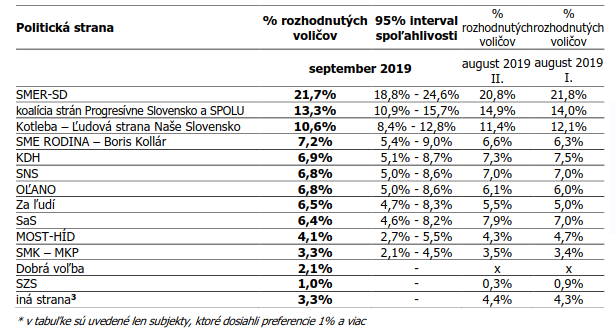
\includegraphics[width=0.8\textwidth]{figs/priklad-focus-prieskumu.png}

Pustili sme sa teda do automatizovaného sťahovania z webu pomocou python knižnice \href{https://github.com/SeleniumHQ/Selenium}{Selenium}. 
Ktorá vie interagovať s webovím prehliadačom ako bežny user. A teda sme pomocou iterativneho odoslania query do prehliadača vo forme: focus prieskum volby {month} {year}" + " filetype:pdf
stiahli prvý result vo forme .pdf filu. Avšak ak v danom mesiaci nebol uskutočnení prieskum stiahli sme file ktorý nám bol zbytočný a museli sme ho identifikovať a odstraniť. 
Podarilo sa nám takýchto reportov získať 127. 


\subsection{Extrahovanie údajov}
Ďalej sme hľadali spôsob ako tieto tabuľky automatizovane extrahovať na účel vytvorenia jednotného .csv súboru.
Použili sme Python knižnicu \href{https://github.com/DS4SD/docling}{Docling}, pomocou ktorej sme prekonvertovali tabuľky z .pdf do pd.DataFrame, spojili a exportovali do jednotného .csv.

Tento proces nebol úplne priamočiary. Názvy politických strán sa extrahovali veľmi nekonzistentne.
Nie len to ale aj fakt, že viaceré politické strany menili meno v priebehu rokov.
Napríklad strana Progresívne Slovensko v roku 2020 kandidovala ako koalícia so stranou SPOLU, avšak v ďalších voľbách už kandidovala iba ako Progresívne Slovensko.
Podobných scénarov bolo viacero, takže sme manuálne vytvorili maper, ktorý tieto názvy zjednotil.
Ďalej bolo potreba niektoré záznamy aj manuálne opraviť, keďže strany s dlhším názvoch (v reporte zabrali dva riadky tabuľky) sa duplikovali v našom extrahovanom datasete.

Po týchto všetkých úkonoch sme už mali jednotný formát dát, ktorý zachytával prieskumy z mnohých mesiacov.

\end{document}
